\documentclass[preview]{standalone}

\usepackage{tikz}
\usetikzlibrary{arrows, calc, angles, quotes, patterns, decorations.pathmorphing, decorations.markings}

\usepackage{xcolor}

\begin{document}
	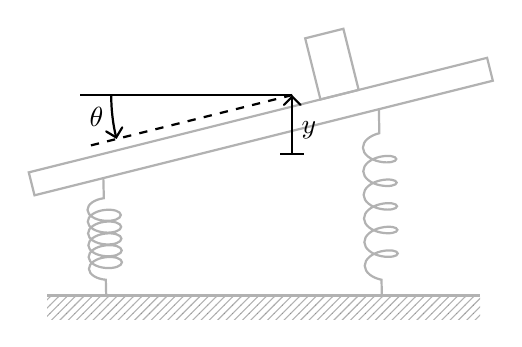
\begin{tikzpicture}[every node/.style={draw, outer sep=0pt, thick}]
	\tikzstyle{spring}=[
		thick,
		decorate,
		decoration={
			coil,
			amplitude = 6pt,
			pre length=0.2cm,
			post length=0.2cm,
			segment length=2mm
		}
	]
	\tikzstyle{damper}=[
		thick,
		decorate,
		decoration={
			markings,  
			mark connection node=dmp,
			mark=at position 0.5 with
			{
				\node (dmp) [thick, inner sep=0pt, transform shape, rotate=-90, minimum width=12pt, minimum height=8pt,draw=none] {};
				\draw [thick] ($(dmp.north east)+(3.5pt,0)$) -- (dmp.south east) -- (dmp.south west) -- ($(dmp.north west)+(3.5pt,0)$);
				\draw [thick] ($(dmp.north)+(0,-4.5pt)$) -- ($(dmp.north)+(0,4.5pt)$);
			}
		}
	]
	\tikzstyle{ground}=[
		fill,
		pattern=north east lines,
		draw=none,
		minimum width=0.75cm,
		minimum height=0.3cm
	]
	
	\node [draw = black!30] (M) [minimum width=6cm, minimum height=0.3cm, rotate=14.03624] {};
	\node [draw = black!30] (m) at ($(M.center)+(1cm,0.405cm)$) [anchor=south, minimum width=0.5cm, minimum height=0.8cm, rotate=14.03624] {};
	
	\node [opacity = 0.3] (ground) at (M.south) [ground, yshift=-2cm, minimum width=5.5cm, anchor=north] {};
	\draw [thick, draw = black!30] (ground.north west) -- (ground.north east);
	
	\coordinate (Atleft) at ($(M.center)+(-2cm,-0.45cm)$);
	\coordinate (Atright) at ($(M.center)+(1.5cm,0.425cm)$);
	
	\draw [spring, draw = black!30, segment length=1.5mm] ($(ground.north)+(-2cm,0)$) -- ($(Atleft)+(0,-0.2cm)$)
		node[midway, xshift=-12pt, draw=none]{};
	\draw [spring, draw = black!30, segment length=3mm] ($(ground.north)+(1.5cm,0)$) --  ($(Atright)+(0,-0.2cm)$)
		node[midway, xshift=12pt, draw=none]{};
		
	\coordinate (CM) at ($(M.center)+(0.4cm,0.4cm)$);
	\coordinate (Bot) at ($(CM)+(-2cm,-0.5cm)$);
	\coordinate (Top) at ($(CM)+(-2.7cm,0)$);
	
	\draw [thick] (CM) ++(-0.15cm,-0.75cm) -- +(0.3cm,0);
	\draw [thick, -angle 90] (CM) ++(0,-0.75cm) -- (CM)
		node[pos=0.4, right, draw=none]{$y$};
		
	\draw [thick] (CM) -- +(-2.70cm,0);
	\draw [thick, dashed, rotate=14.03624] (CM) -- +(-2.70cm,0);
		
	\pic [draw, -angle 90, "$\theta$" {draw=none, left}, angle eccentricity=1, angle radius=2.3cm] {angle = Top--CM--Bot};
	\end{tikzpicture}
\end{document}